\documentclass[../main.tex]{subfiles}


\begin{document}

\subsection*{(a)}
After importing the situation table from Celonis into RapidMiner we can design the decision tree learning process using the cross validation operator after setting the class variable: \\
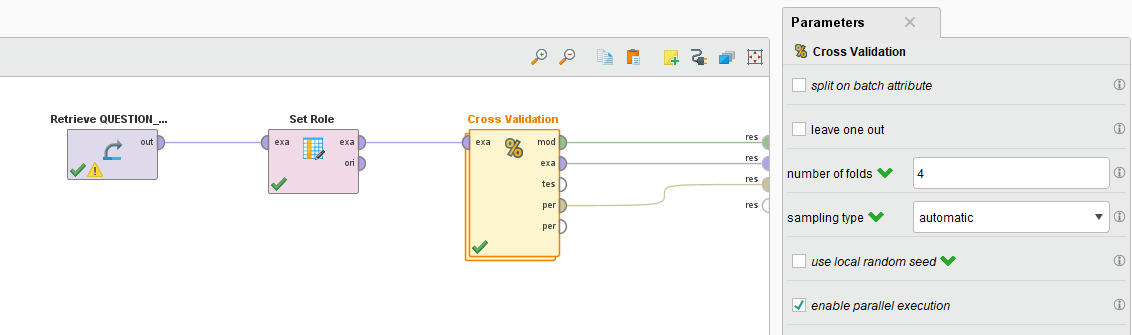
\includegraphics[width=\textwidth]{img/RapidMiner_Process_Overview.png}

We construct the training section of the cross validation using the decision tree operator in RapidMiner and also specifying the given parameters. In the testing section we simply apply the current test set to the given model and run a performance check upon it. \\
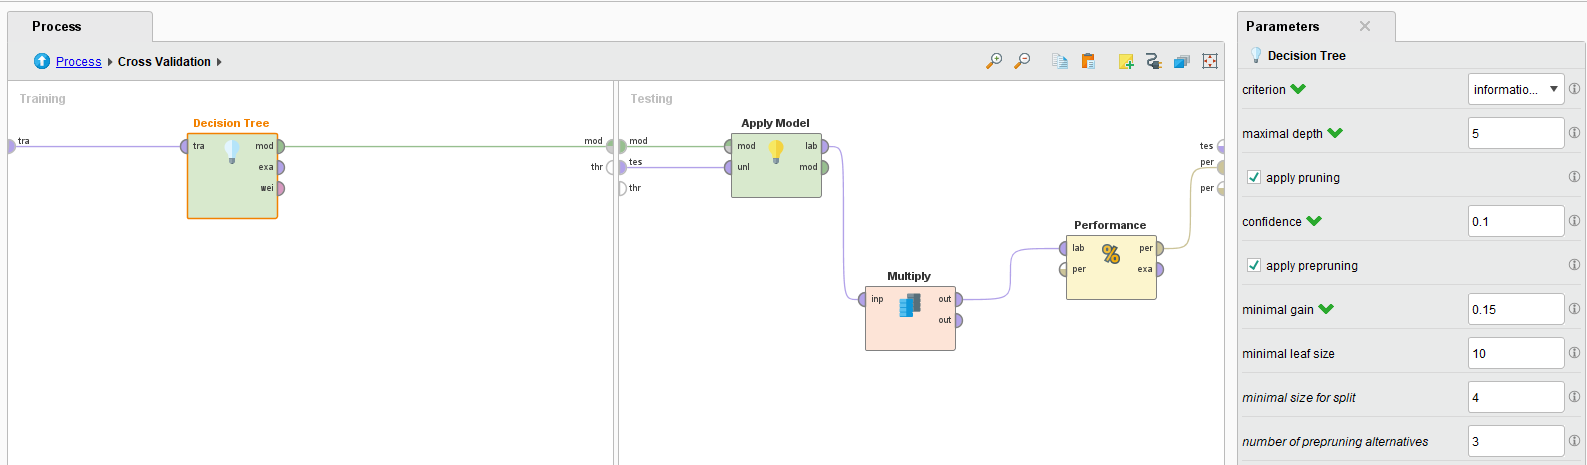
\includegraphics[width=\textwidth]{img/RapidMiner_Process_Cross_Validation.png}

This process results in the following decision tree: \\
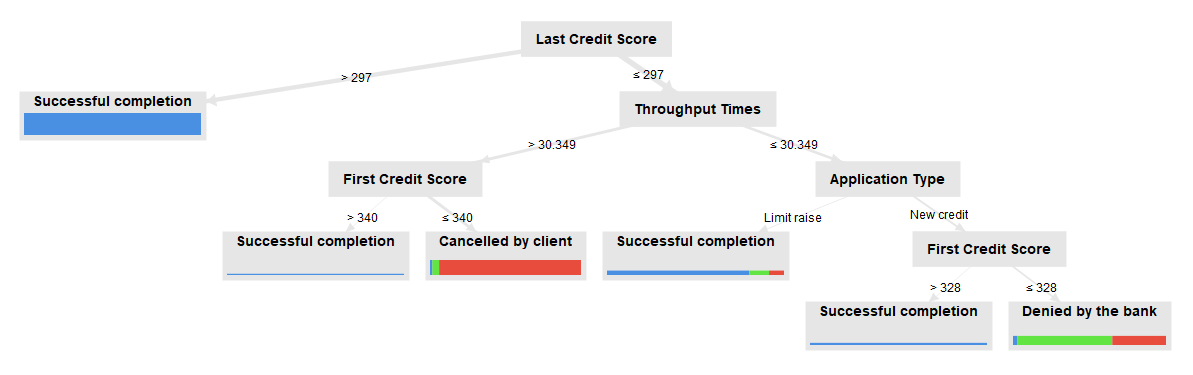
\includegraphics[width=\textwidth]{img/RapidMiner_Results_Decision_Tree.png}

Here we can see that for all applications, where the applicants last credit score was above $297$, the application was successfully completed.

We can also observe, that the very few applicants for new credits, those credit scores dropped significantly (First Credit Score $> 329$ and Last Credit Score $\leq 297$) within a time less or equal to $30.349$ days, all completed their application successfully.

Using the cross validation operator, we could also observe the following performance metrics: \\
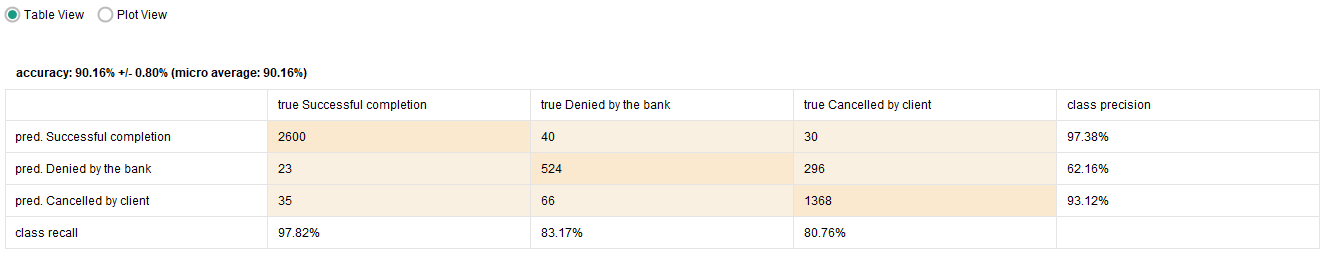
\includegraphics[width=\textwidth]{img/RapidMiner_Results_Performance.png}

\subsection*{(b)}
\begin{enumerate}
	\item	Most applicants with a last credit score of at most $297$ cancelled their own application when it was already roughly over a month's time in progress. Perhaps the current application process needs to be revised to minimize throughput times.
	\item	$62\%$ of applications, that was roughly under a months time in progress, by applicants with a last credit score of at most $297$ for a new credit were rejected by the bank, if their first credit score was at most $328$. If the bank seeks for more successful application completions, perhaps they should adjust their rejection criteria.
\end{enumerate}

\end{document}